\documentclass[border=2mm]{standalone}
\usepackage{tikz}
\usepackage{pgfplots}
\usepackage{amsmath}
\pgfplotsset{compat=1.18}

% Definición de colores según paleta identificada
\definecolor{pais1color}{HTML}{00CED1}  % Cyan - País 1
\definecolor{pais2color}{HTML}{000000}  % Negro - País 2
\definecolor{pais3color}{HTML}{8B4513}  % Marrón - País 3
\definecolor{pais4color}{HTML}{00CED1}  % Cyan - País 4
\definecolor{pais5color}{HTML}{FF8C00}  % Naranja - País 5
\definecolor{gridcolor}{HTML}{CCCCCC}   % Gris claro - Grilla

\begin{document}
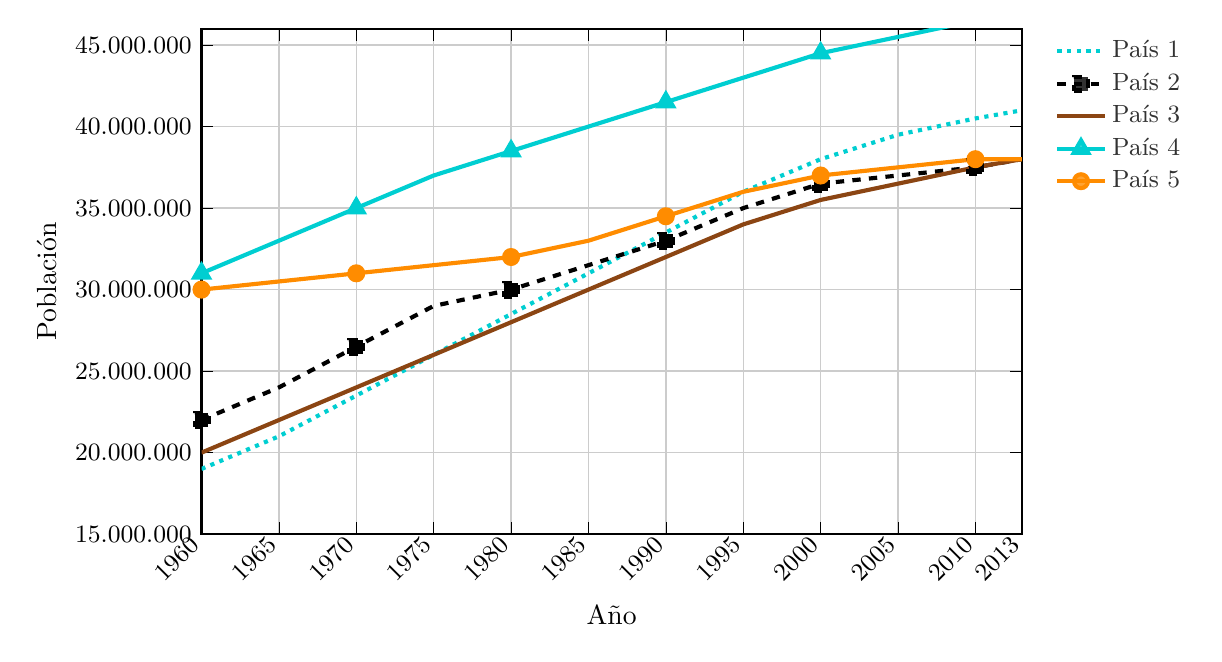
\begin{tikzpicture}
\begin{axis}[
    % Configuración de ejes
    xlabel={Año},
    ylabel={Población},
    xmin=1960, xmax=2013,
    ymin=15000000, ymax=46000000,
    % Ticks del eje X - Sin separador de miles para años
    xtick={1960,1965,1970,1975,1980,1985,1990,1995,2000,2005,2010,2013},
    xticklabel style={rotate=45, anchor=east, font=\small, /pgf/number format/.cd, 1000 sep={}},
    % Ticks del eje Y con formato de millones
    ytick={15000000,20000000,25000000,30000000,35000000,40000000,45000000},
    yticklabels={15.000.000, 20.000.000, 25.000.000, 30.000.000, 35.000.000, 40.000.000, 45.000.000},
    yticklabel style={font=\small},
    scaled y ticks=false,
    % Grilla
    grid=major,
    grid style={gridcolor, line width=0.5pt},
    % Dimensiones del gráfico
    width=12cm,
    height=8cm,
    % Leyenda
    legend pos=outer north east,
    legend style={
        font=\small,
        draw=none,
        fill=white,
        fill opacity=0.8
    },
    % Estilo de ejes
    axis lines=box,
    axis line style={black, line width=0.8pt},
    tick style={black},
]

% País 1 - Línea punteada cyan (sin marcadores)
% Datos aproximados de la imagen: crecimiento desde ~19M a ~41M
\addplot[
    color=pais1color,
    line width=1.5pt,
    dotted,
    mark=none,
] coordinates {
    (1960, 19000000)
    (1965, 21000000)
    (1970, 23500000)
    (1975, 26000000)
    (1980, 28500000)
    (1985, 31000000)
    (1990, 33500000)
    (1995, 36000000)
    (2000, 38000000)
    (2005, 39500000)
    (2010, 40500000)
    (2013, 41000000)
};
\addlegendentry{País 1}

% País 2 - Línea discontinua negra con marcadores cuadrados
% Datos aproximados: crecimiento desde ~22M a ~38M
\addplot[
    color=pais2color,
    line width=1.5pt,
    dashed,
    mark=square*,
    mark size=2.5pt,
    mark repeat=2,
] coordinates {
    (1960, 22000000)
    (1965, 24000000)
    (1970, 26500000)
    (1975, 29000000)
    (1980, 30000000)
    (1985, 31500000)
    (1990, 33000000)
    (1995, 35000000)
    (2000, 36500000)
    (2005, 37000000)
    (2010, 37500000)
    (2013, 38000000)
};
\addlegendentry{País 2}

% País 3 - Línea sólida marrón (sin marcadores)
% Datos aproximados: crecimiento desde ~20M a ~38M
\addplot[
    color=pais3color,
    line width=1.5pt,
    solid,
    mark=none,
] coordinates {
    (1960, 20000000)
    (1965, 22000000)
    (1970, 24000000)
    (1975, 26000000)
    (1980, 28000000)
    (1985, 30000000)
    (1990, 32000000)
    (1995, 34000000)
    (2000, 35500000)
    (2005, 36500000)
    (2010, 37500000)
    (2013, 38000000)
};
\addlegendentry{País 3}

% País 4 - Línea sólida cyan con marcadores triangulares
% Datos aproximados: crecimiento desde ~31M a ~47M (mayor crecimiento)
\addplot[
    color=pais4color,
    line width=1.5pt,
    solid,
    mark=triangle*,
    mark size=3pt,
    mark repeat=2,
] coordinates {
    (1960, 31000000)
    (1965, 33000000)
    (1970, 35000000)
    (1975, 37000000)
    (1980, 38500000)
    (1985, 40000000)
    (1990, 41500000)
    (1995, 43000000)
    (2000, 44500000)
    (2005, 45500000)
    (2010, 46500000)
    (2013, 47000000)
};
\addlegendentry{País 4}

% País 5 - Línea sólida naranja con marcadores circulares
% Datos aproximados: relativamente estable desde ~30M a ~38M
% Se cruza con País 2 aproximadamente en 1998
\addplot[
    color=pais5color,
    line width=1.5pt,
    solid,
    mark=*,
    mark size=2.5pt,
    mark repeat=2,
] coordinates {
    (1960, 30000000)
    (1965, 30500000)
    (1970, 31000000)
    (1975, 31500000)
    (1980, 32000000)
    (1985, 33000000)
    (1990, 34500000)
    (1995, 36000000)
    (2000, 37000000)
    (2005, 37500000)
    (2010, 38000000)
    (2013, 38000000)
};
\addlegendentry{País 5}

\end{axis}
\end{tikzpicture}
\end{document}
